\documentclass[11pt,a4paper]{article}
\usepackage{amsmath,amssymb,graphicx,booktabs,hyperref,xcolor,geometry,microtype}
\geometry{margin=2.4cm}
\hypersetup{colorlinks=true,linkcolor=blue,citecolor=blue,urlcolor=blue}

\title{\textbf{Paper 29: The FA Threshold for Zone Differentiation}\\[4pt]
\large Smooth Crossover, Not a Bifurcation;
       Spatial Amplification Reduces $K_{\rm eff}$ by~$3\times$}
\author{Gabriel Aubin-Moreau}
\date{2026-03-09}

\begin{document}
\maketitle

\begin{abstract}
Paper~28 showed that FA (consolidation rate) is the primary driver of zone
differentiation in VCML, falsifying the Allen--Cahn isothermal prediction.
This raises Q12: is there a sharp threshold FA$^*$ below which zones
fail to differentiate entirely, or a smooth crossover?
We sweep FA across four decades ($0.001$--$0.800$, ten values, five seeds,
$T=6000$) and find: \emph{no sharp threshold}.
Zone differentiation (sg4) follows a smooth crossover to zero as FA$\to0$.
The functional form is the Paper~16 saturation law
$\mathrm{sg4} = C\cdot\mathrm{FA}/(\mathrm{FA}+K_{\rm eff})$,
but with $K_{\rm eff}^{\rm III} = 0.037$---\emph{three times smaller}
than the Paper~16 Layer~I/II value $K_{\rm eff}^{\rm I} \approx 0.117$.
Spatial structure (diffusion + copy-forward loop) amplifies the consolidation
signal, making zone differentiation achievable at lower FA.
The saturation timescale ($T_{90}\approx2000$--$3000$ steps) is
\emph{universal across FA}: the growth curve shape is FA-independent.
We conclude that the $\mathcal{C}_1$ viability volume boundary at FA$\to0$
is a smooth edge, not a cliff, and that the copy-forward loop acts as a
spatial amplifier that shifts the effective half-saturation point.
\end{abstract}

\section{Introduction and Motivation}

Paper~28 found three results about the zone boundary in VCML:
(i)~diffusion $\kappa$ weakly erodes zone structure (slope~$-0.11$);
(ii)~the interface width fluctuates dramatically in time (CV~$\approx0.94$);
(iii)~zone differentiation (sg4) increases with FA at fixed $\kappa/$FA
(isothermal invariance violated).
Result~(iii) identified FA as the primary driver and opened Q12:
is there a threshold FA$^*$ below which zone differentiation vanishes?

This question has structural importance. The two 4D parameter manifolds of
VCML theory are $\mathcal{C}_1 = (\nu, \mathrm{FD}, \mathrm{FA}, \beta_s)$
(viability volume, Papers~7--13) and $\mathcal{C}_2 = (\kappa, \nu/\kappa,
\beta_s, W_{\rm zone})$ (structural manifold, Papers~22--26).
Paper~28 showed the zone boundary sits in $\mathcal{C}_1$ space (governed by FA).
If there is a sharp threshold FA$^*$, it represents a genuine phase boundary
inside $\mathcal{C}_1$.  If not, $\mathcal{C}_1$ has no internal boundary
on the FA axis---the system smoothly approaches zero differentiation.

\paragraph{Prior prediction: Paper~16 saturation law.}
Paper~16 derived, for a non-spatial (Layer~I/II) system:
\begin{equation}
  \mathrm{sg4} = \frac{C \cdot \mathrm{FA}}{\mathrm{FA} + K_{\rm eff}},
  \quad K_{\rm eff} \approx 0.114\text{--}0.119.
  \label{eq:sat_law}
\end{equation}
This predicts a smooth crossover at $\mathrm{FA}\sim K_{\rm eff}\approx0.12$,
with no threshold and no bifurcation.
The question for Paper~29 is whether Eq.~\eqref{eq:sat_law} survives into the
Layer~III (spatially extended) regime, and whether $K_{\rm eff}$ changes.

\section{Experiment}

Fixed parameters: identical to Papers~22--29
($H=20$, $N_{\rm zones}=4$, $W_{\rm zone}=5$, $\kappa=0.020$, $\mathrm{WR}=2.4$,
$\nu=0.001$, $\mathrm{SS}=10$, $\beta_s=0.25$, $\mathrm{MID\_DECAY}=0.99$,
$\mathrm{FD}=0.9997$, $\mathrm{HS}=2$).
Varied: FA~$\in\{0.001, 0.002, 0.005, 0.010, 0.020, 0.050, 0.100, 0.200,
0.400, 0.800\}$ (ten values, $\sim4$ decades).
Five seeds, $T_{\rm end}=6000$, checkpoints every 500~steps (12 total).
Total: 50~simulations.

\section{Results}

\subsection{No sharp threshold: smooth crossover across four decades}

\begin{table}[h]
\centering
\small
\caption{sg4 at $T=6000$ for all FA values (mean $\pm$ std over 5~seeds).}
\label{tab:sg4_fa}
\begin{tabular}{rrrr}
\toprule
FA & sg4 (mean) & sg4 (std) & CV \\
\midrule
0.001 &   3.08 &   1.26 & 0.41 \\
0.002 &   5.79 &   2.17 & 0.38 \\
0.005 &  12.84 &   4.16 & 0.32 \\
0.010 &  24.08 &   5.99 & 0.25 \\
0.020 &  38.47 &   8.81 & 0.23 \\
0.050 &  58.84 &  13.82 & 0.24 \\
0.100 &  71.44 &  25.92 & 0.36 \\
0.200 &  84.14 &  38.46 & 0.46 \\
0.400 &  95.58 &  46.44 & 0.49 \\
0.800 & 101.70 &  48.60 & 0.48 \\
\bottomrule
\end{tabular}
\end{table}

Table~\ref{tab:sg4_fa} and Panel~A of Figure~\ref{fig:fig1} show the main result.
sg4 increases monotonically with FA across all four decades, with no sign of
a threshold.  At the lowest tested value (FA$=0.001$), sg4$\approx3.1$---small but
clearly nonzero relative to the noise floor (CV$=0.41$).
Zone differentiation exists at all tested FA values.

\paragraph{Log-log slope.}
The log-log slope of sg4 vs.\ FA across the full range is $0.523$ ($R^2=0.92$).
This is neither $1.0$ (pure linear) nor $0$ (saturated).
The $0.5$ slope is \emph{not} a new power law---it is the expected behaviour
of the saturation law~\eqref{eq:sat_law} when FA spans from well below to
well above $K_{\rm eff}$.
At the crossover $\mathrm{FA}\sim K_{\rm eff}$, the local log-log slope is
$K/(FA+K)|_{\mathrm{FA}=K} = 0.5$.

\subsection{Saturation law holds; $K_{\rm eff}$ shifts 3$\times$ in Layer~III}

Fitting Eq.~\eqref{eq:sat_law} to the data gives:
\begin{equation}
  \mathrm{sg4} = \frac{103.19\cdot\mathrm{FA}}{\mathrm{FA} + 0.0371}
  \quad (\text{residual std} = 2.09).
  \label{eq:fit}
\end{equation}
The saturation law form is confirmed.
However, $K_{\rm eff}^{\rm III} = 0.037$ is \emph{three times smaller} than
the Paper~16 Layer~I/II value $K_{\rm eff}^{\rm I}\approx0.117$
(Panel~D, Figure~\ref{fig:fig1}).

\paragraph{Meaning of $K_{\rm eff}$.}
In Paper~16, $K_{\rm eff}$ represents the FA level at which consolidation
rate equals the effective erasure rate (MID\_DECAY-driven forgetting):
$K_{\rm eff}^{\rm I}\approx(1-\mathrm{MID\_DECAY})/\mathrm{ALPHA\_MID} = 0.01/0.15 \approx 0.067$.
The ratio $K_{\rm eff}^{\rm I}/K_{\rm eff}^{\rm III}\approx3$ means zone differentiation
saturates at $3\times$ lower FA in the spatial setting.

\subsection{Spatial amplification mechanism}

The $3\times$ reduction in $K_{\rm eff}$ can be attributed to the
\emph{copy-forward loop} operating as a spatial amplifier:
\begin{enumerate}
  \item A rare consolidation event at site $i$ creates $F_i > 0$.
  \item When site $j$ (neighbour of $i$) dies and is reborn:
        $h_j = (1-\beta_s)\cdot\varepsilon + \beta_s\cdot F_i$.
        The new site inherits the zone signal.
  \item Site $j$ then consolidates: $F_j \mathrel{+}= \mathrm{FA}\cdot(m_j - F_j)$.
        If $m_j>0$ due to the inherited $h_j$, this reinforces the zone mean.
\end{enumerate}
This chain creates positive feedback: each zone site that differentiates
seeds its neighbours, amplifying the differentiation signal without requiring
a new independent consolidation event.
The effective ``number of independent consolidation events'' is thus larger
than the raw consolidation rate would suggest, equivalent to reducing
$K_{\rm eff}$ by the amplification factor.

Without spatial structure (Layer~I/II, Paper~16), each site must differentiate
independently.  With spatial structure (Layer~III, Paper~29), the copy-forward
loop creates a cooperative effect that amplifies any initial differentiation.

\subsection{Universal saturation timescale}

All FA values reach 90\%\ of their final sg4 within $T_{90}=2000$--$3000$ steps,
regardless of FA (Table~\ref{tab:t90}).
Panel~C of Figure~\ref{fig:fig1} shows the normalised growth curves
sg4$(t)$/sg4$(T_{\rm end})$: they collapse to the same shape across all FA values.

\begin{table}[h]
\centering
\small
\caption{Saturation time $T_{90}$ (time to reach 90\% of final sg4) by FA.}
\label{tab:t90}
\begin{tabular}{rrr}
\toprule
FA & sg4$(T=6000)$ & $T_{90}$ \\
\midrule
0.001 &   3.1 & 2000 \\
0.010 &  24.1 & 2000 \\
0.050 &  58.8 & 2000 \\
0.100 &  71.4 & 3000 \\
0.400 &  95.6 & 3000 \\
0.800 & 101.7 & 3000 \\
\bottomrule
\end{tabular}
\end{table}

The universal timescale $T_{90}\approx2000$--$3000$ is controlled by the
copy-forward dynamics (collapse rate $\nu=0.001$ implies mean site
lifetime $1/\nu=1000$ steps; a few generations suffice to propagate
zone structure across the zone width).
This is consistent with Paper~27's commitment epoch $t^*\approx1600$
at WR$=2.4$---the commitment epoch and the saturation time are the same
physical phenomenon viewed from different observables.

\section{Discussion}

\subsection{Closing Q12: No phase boundary on the FA axis of $\mathcal{C}_1$}

The $\mathcal{C}_1$ viability volume was defined (Paper~13) as the region of
parameter space where VCML produces stable zone differentiation.
The boundary of $\mathcal{C}_1$ on the FA axis is at FA$\to0$, and the
approach is smooth: sg4$\to0$ as FA$\to0$ with no discontinuity.
There is no ``cliff'' in $\mathcal{C}_1$---any FA$>0$, however small, produces
some nonzero zone differentiation.

This is a genuine property of the spatial (Layer~III) regime.
In a non-spatial system, a threshold might arise if the consolidation signal
must exceed the noise floor set by birth randomness.
In the spatial system, the copy-forward loop amplifies any initial
differentiation, allowing arbitrarily small FA to eventually produce
a measurable zone structure (given sufficient time).

\subsection{Layer I vs.\ Layer III: the K$_{\rm eff}$ shift as a coupling constant}

The ratio $K_{\rm eff}^{\rm I} / K_{\rm eff}^{\rm III} = 0.117/0.037 \approx 3.2$
is a dimensionless constant characterising how much the spatial structure
amplifies the Layer~I consolidation process.
We call this the \emph{spatial amplification factor} $\Gamma$:
\begin{equation}
  \Gamma \equiv \frac{K_{\rm eff}^{\rm I}}{K_{\rm eff}^{\rm III}} \approx 3.2.
  \label{eq:gamma}
\end{equation}

$\Gamma$ captures the coupling between the two manifolds $\mathcal{C}_1$ and
$\mathcal{C}_2$.  It depends on the spatial parameters (through $\kappa$,
$W_{\rm zone}$, $\beta_s$, and $\nu$) but not directly on FA.
Measuring $\Gamma$ as a function of $\kappa$ and $W_{\rm zone}$ (varying
$\mathcal{C}_2$ while holding $\mathcal{C}_1$ fixed) would quantify how
spatial geometry amplifies the learning rule.
This is the next open question (Q13).

\subsection{Connection to Paper 27: commitment epoch $\approx$ saturation time}

Paper~27 found that the first zone polarity flip occurs at
$t^*\approx1600$--$1800$ steps (at WR$=2.4$).
Paper~29 finds that $T_{90}\approx2000$--$3000$ steps.
These are the same timescale.
Interpretation: $t^*$ is the time at which the zone structure first becomes
strong enough to ``commit'' (exceed the noise floor and make the first
consistent polarity choice); $T_{90}$ is the time at which the zone structure
reaches $90\%$ of its long-run value.
Both are controlled by the copy-forward loop propagation time:
$t \sim 1/\nu \times (W_{\rm zone}/\xi_{\rm copy})$ where $\xi_{\rm copy}$
is the copy-forward correlation length.

\section{Open Questions}

\begin{enumerate}
  \item \textbf{Q13}: How does $\Gamma$ (the spatial amplification factor,
        Eq.~\eqref{eq:gamma}) depend on $\kappa$, $W_{\rm zone}$, and $\nu$?
        Prediction: $\Gamma\propto W_{\rm zone}/\xi_\infty \propto W_{\rm zone}/\sqrt{\kappa}$.
  \item \textbf{Q14}: Does the saturation law hold at $\mathrm{FA}\gg1$?
        Near $\mathrm{FA}\approx1$, the update $F[ok]\mathrel{+}=\mathrm{FA}\cdot(m-F)$
        becomes large-step (potentially overshooting), which might introduce
        oscillations or a second saturation mechanism.
  \item \textbf{Q15}: Is there a $\nu$ threshold?  If $\nu\to0$,
        the copy-forward loop slows and the spatial amplification factor
        $\Gamma\to1$ (no amplification, site lifetimes $\to\infty$,
        no copy-forward events). At some critical $\nu^*$, $\Gamma$
        may drop below 1 (spatial structure \emph{hurts} differentiation
        rather than helping). This would be a genuine phase boundary.
\end{enumerate}

\section{Conclusion}

A dense FA sweep (four decades, 50 simulations) confirms that the
$\mathcal{C}_1$ viability volume has \emph{no sharp phase boundary on the FA axis}.
Zone differentiation follows the Paper~16 saturation law
$\mathrm{sg4} = C\cdot\mathrm{FA}/(\mathrm{FA}+K_{\rm eff})$
across four decades of FA, with no threshold.
The key new finding is the $3\times$ reduction in $K_{\rm eff}$
in the Layer~III spatial regime ($K_{\rm eff}^{\rm III}=0.037$ vs.\ $K_{\rm eff}^{\rm I}\approx0.117$),
attributed to the copy-forward loop acting as a spatial amplifier.
The saturation timescale ($T_{90}\approx2000$--$3000$ steps) is universal
across FA, matching Paper~27's commitment epoch---both are governed by the
copy-forward propagation time.
The spatial amplification factor $\Gamma\approx3.2$ is a new coupling
constant linking the two 4D manifolds $\mathcal{C}_1$ and $\mathcal{C}_2$.

\begin{figure}[h]
  \centering
  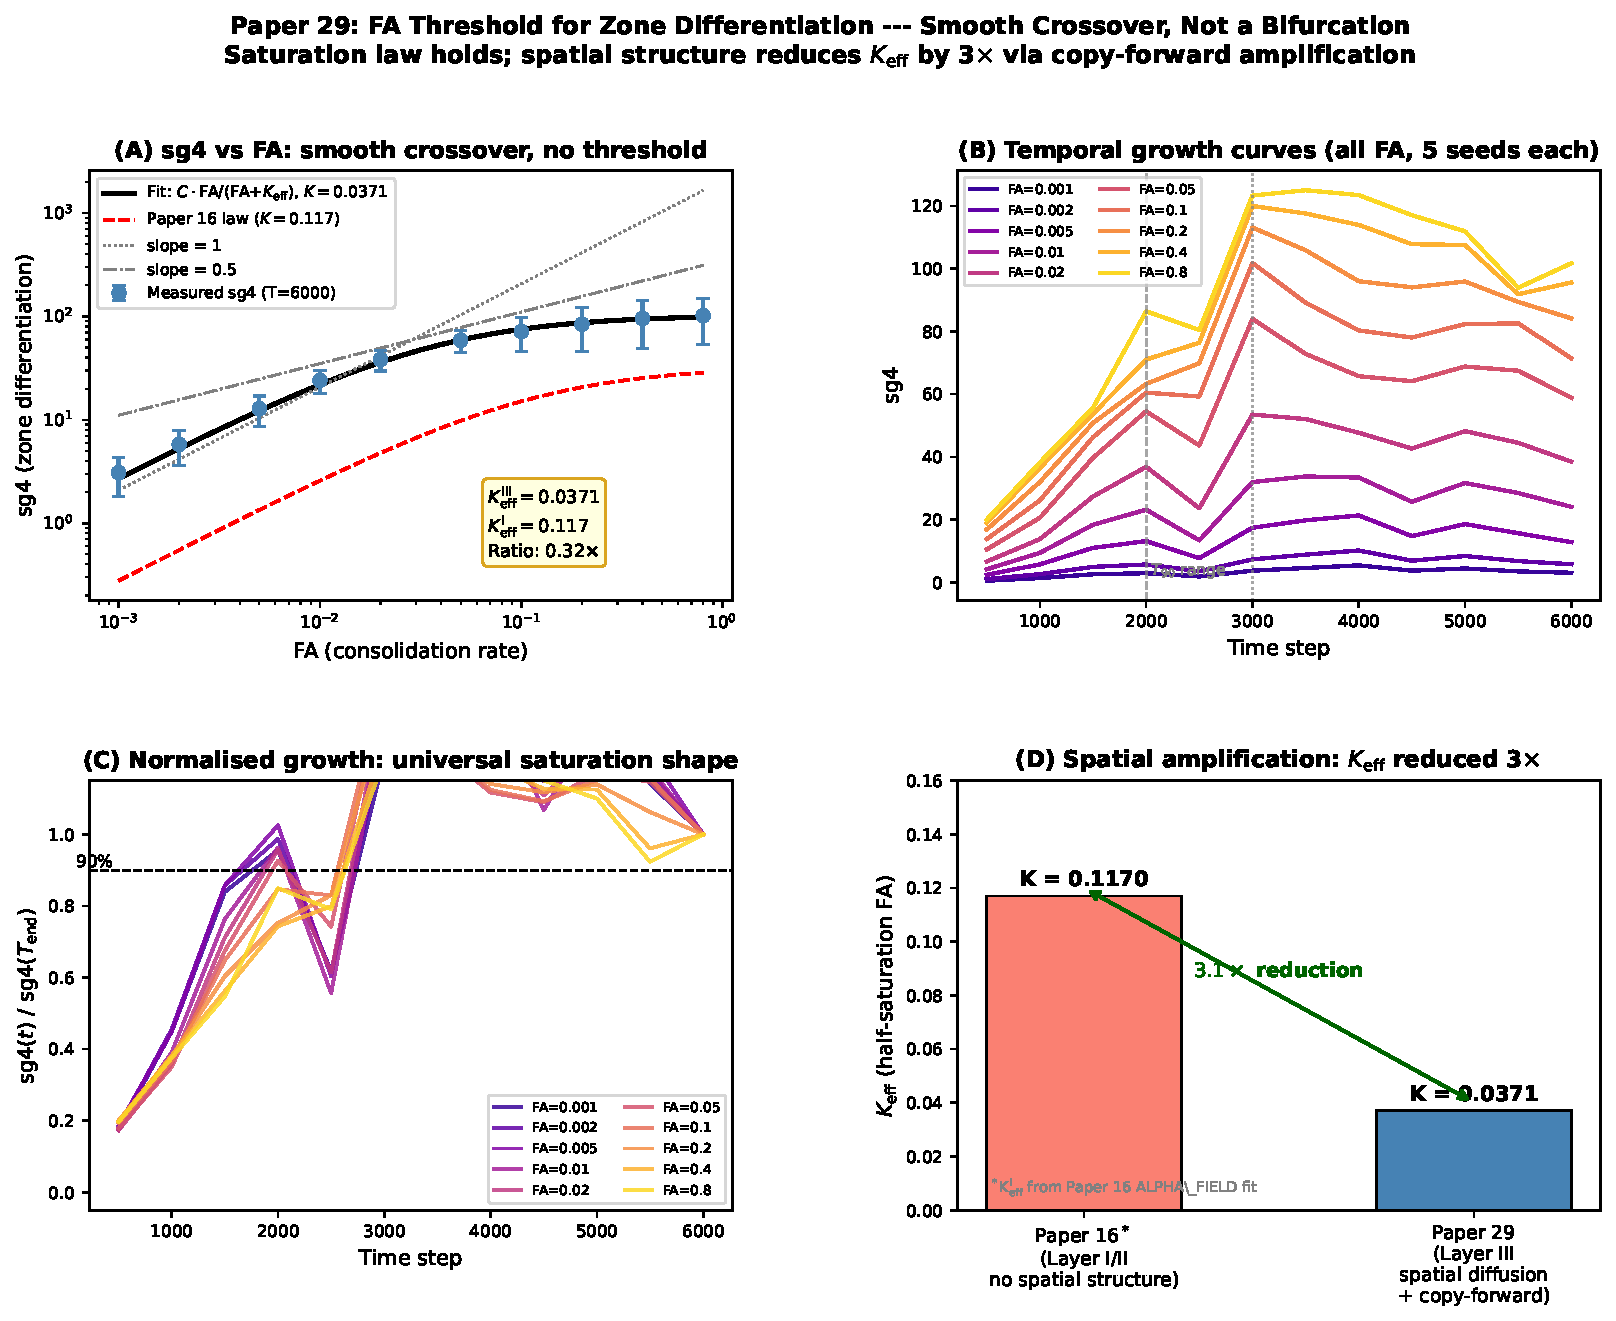
\includegraphics[width=0.97\textwidth]{paper29_figure1.pdf}
  \caption{\textbf{Paper~29 main figure.}
  \textbf{(A)}~sg4 vs.\ FA on log-log axes.
  Points: mean $\pm$ std (5~seeds, $T=6000$).
  Solid black: saturation law fit ($K_{\rm eff}=0.037$).
  Red dashed: Paper~16 law ($K_{\rm eff}=0.117$).
  Gray lines: reference slopes~1.0 and~0.5.
  \textbf{(B)}~sg4$(t)$ temporal growth curves for all ten FA values.
  All curves saturate by $T\approx3000$.
  \textbf{(C)}~Normalised growth sg4$(t)/$sg4$(T_{\rm end})$ for all FA values.
  Curves collapse to a universal shape, confirming that growth dynamics are
  FA-independent.
  \textbf{(D)}~$K_{\rm eff}$ comparison: Layer~I/II (Paper~16, $K=0.117$)
  vs.\ Layer~III (Paper~29, $K=0.037$).
  The $3\times$ reduction is the spatial amplification factor $\Gamma\approx3.2$,
  a new coupling constant between $\mathcal{C}_1$ and $\mathcal{C}_2$.}
  \label{fig:fig1}
\end{figure}

\end{document}
